\documentclass[10pt]{article}
\usepackage{fullpage,enumitem,amsmath,amssymb,graphicx,setspace,float, multicol,epstopdf}

%\setlength{\parskip}{-0.5\baselineskip}%
%\setlength{\parindent}{0cm}
\singlespacing

\begin{document}
\title{CS 224W Project Report\\ The Evolution of Wikipedia}
\author{Jiaji Hu, Haozhun Jin, Peng Qi\\Group \#48}
\date{}
\maketitle

\begin{multicols}{2}
\section{Introduction}

The evolution of online networks is a topic that has generated much interest in research. In the past, scientists have studied some dynamic properties of network evolution, choosing to focus on online social networks and proposing a variety of models with some degree of success. However, much is yet to be learned about how large networks grow and evolve.

As the largest online encyclopedic resource in human history, Wikipedia is an interesting example of an online network. Unlike social networks --- the usual object of analysis, Wikipedia is a knowledge network, representing the structure of information instead of social relationships. Therefore, studying the dynamics of Wikipedia can be a refreshing addition to network evolution reasearch.

In our project, we studied the evolution of Wikipedia on both static and dynamic viewpoints. Using data that consists of Wikipedia's complete edit history, we took snapshots of Wikipedia at different timepoints and compute statistics to looked for trends over time and gained insight into the network structure. By comparing snapshots taken between a short period of time, we single out individual edge creation processes and study them, focusing on the choice of destination for new edges. On our Wikipedia network, we compare and evaluate previous edge destination models such as the triangle closing model and models based on Preferential Attachment. From this, we go on to propose that new edges not only choose their destinations according to the degree of a destination node, but also according to the PageRank score of that destination. We evaluate the effectiveness of PageRank as a predictor of edge destination, comparing it to node degree. From our project, we hope to find out both results that reveal interesting information about Wikipedia in particular, and results that apply to network evolution in general.

\section{Prior Work}

In recent years, researchers have done a considerable amount of work on modeling the evolution of networks. In the process, both static and dynamic means of analysis have been used.

Static analysis consists of taking snapshots of the network at different stages of its development and computing statistical properties of interest for each snapshot to reach a conclusion to the process of network evolution. In \cite{kumar2010structure}, the authors took snapshots to analyze the structural properties of their network, focusing on the size of each connected component. In \cite{zlatic2011model}, the authors use snapshots to compute reciprocity of edges, arriving at conclusions about the structure of Wikipedia. However, using their model, the intermediate status of the graph in the process of generation does not match to any time point of the real graph. Only the final state of the generated graph matches the real-world graph in some characteristics.

On the other hand, research taking the dynamic view do not rely on snapshots, but rather studies the change in network on an edge-by-edge basis. In \cite{leskovec2008microscopic}, the authors studied the exact edge arrival sequence to directly observe and model the fine-grain evolution process of networks. The paper considered dynamic analysis to be made up of three core processes: node arrival, edge initiation and edge destination. In particular, edge initiation and edge destination were closely studied, and a random-random triangle closing model was proposed as a good model for predicting edge destination.

The preferential attachment (PA) theory was proposed and evaluated in both \cite{leskovec2008microscopic} and \cite{zlatic2011model}. In \cite{leskovec2008microscopic}, PA was evalutated dynamically on social networks, while in \cite{zlatic2011model}, it was analyzed with a static view on Wikipedia data. This project will combine the two and assess preferential attachment with a dynamic point of view on the Wikipedia dataset, so as to further evaluate the validity of this theory.

We see that most papers in this field, including \cite{leskovec2008microscopic}, \cite{kossinets2006empirical} and \cite{kumar2010structure} were written with social networks as the object of study. This raises the question whether their proposed models hold in other types of networks. This paper aims to explore some of these models on Wikipedia to answer this question.

\section{Model}
We model Wikipedia as an unweighted directed graph where each document is a node, and each edge $\langle u, v \rangle$ represents that there exists referential link from document $u$ to document $v$. We model Wikipedia as unweighted for model simplicity, which means we choose to ignore the fact that some documents $u$ might link to some other document $v$ multiple times.


\section{Data Collection and\\ Processing}
Wikipedia offers free copies of its contents for mirrors and research. In most of the use cases, a snapshot is enough. But for the purpose of our project, we need the edit history. Therefore we chose the {\it pages-meta-history} dataset, which contains the complete edit history. We used the August 2006 version of English Wikipedia from the official Wikimedia archives.

The dump is more than 720GB after decompression. To reduce the time cost of processing such data, for each article and for each revision, we extracted the article title, its list of outgoing links and time of revision. Next, we assigned each article an id to further minimize file sizes. This gave us a boiled down version of the information we needed. From there, we sorted all revisions along with the article id and ids of articles it links to by the revision time. After that, we were ready to generate snapshots of the Wikipedia graph over time.

Due to special characteristics of Wikipedia, we also did some additional preprocessing. For one, we removed all articles with a colon in its name. These articles were in special namespaces, serving as talk pages, user pages, images, or special administrative pages, etc. Such pages are not in our interest.

Also, redirections in Wikipedia may have a special effect on the graph. We decided to study this effect. To construct a redirection-free version of the graph, we removed all articles that redirected to another in the snapshots. After the removal, we moved all relevant edges to the page that it was redirected to. We noticed a very small portion of redirections that turned into a cycle. Such pages were removed completely.

\section{Snapshot Analysis}
A snapshot is a static view of an evolving network at a certain point in time. After generating a snapshot, we can do static analysis of its properties. In our project, we looked at the following properties of each snapshot:
\begin{enumerate}
\item Number of nodes and edges.
\item Degree distributions, including in-degree and out-degree.
\item Diameter (sampling from a subset of nodes for efficiency).
\item Connected component sizes.
\end{enumerate}

Looking at these properties for each snapshot gives us an idea about the structure of the graph at that time. By comparing these statistics over many snapshots through time, we look for trends as the network develops. The interval between snapshots was chosen so that the snapshots are close enough to fully present the developmental stages of the network. The results are as follows:

\subsection{Number of Nodes and Edges}
From Fig.~\ref{fig:growth}, it is evident that Wikipedia network grows almost exponentially over time in terms of both node number and edge number (especially after 2003). It it further observed that the number of Wikipedia's nodes and edges grow by one order (10x) in about 22 months. Fig.~\ref{fig:growth} shows that the ratio of nodes to edges roughly follow a linear pattern throughout Wikipedia's growth.

A closer observation on the linear scale graph revealed a significant difference in node count before and after (marked with ``(R)'' in the graphs) our redirection process, which is intuitively correct as it removes conceptually redundant nodes and edges. As for edge/node ratio, after processing redirection, the edge/node ratio still follows a roughly linear growth, which indicates that the ratio of redirection nodes in the corpus is roughly constant.

\begin{figure*}
\centering{
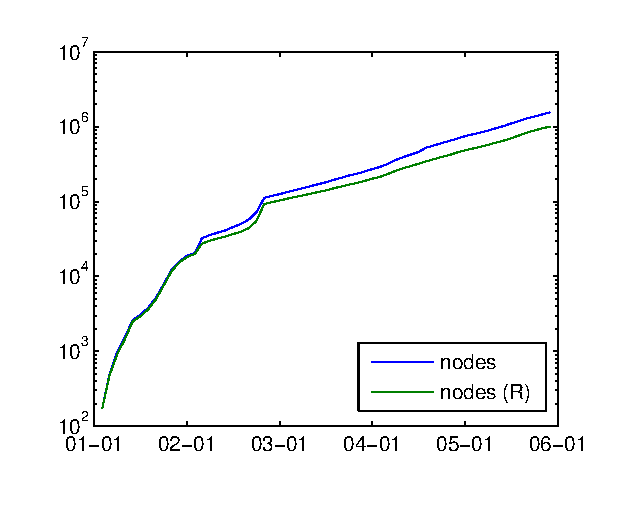
\includegraphics[width=0.3\textwidth]{./graphs/p1-1}
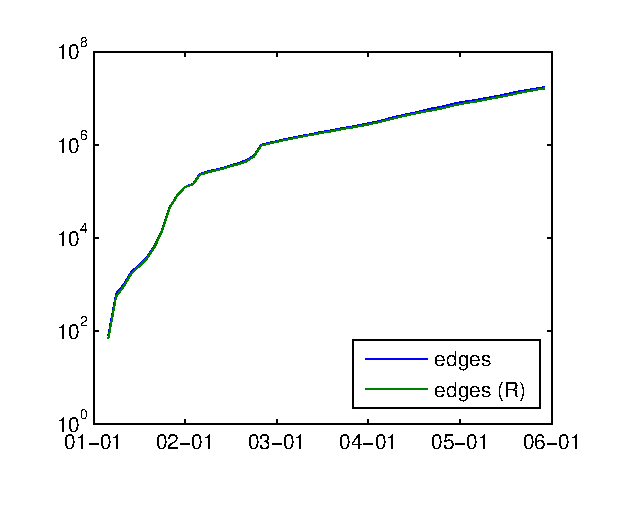
\includegraphics[width=0.3\textwidth]{./graphs/p1-2}
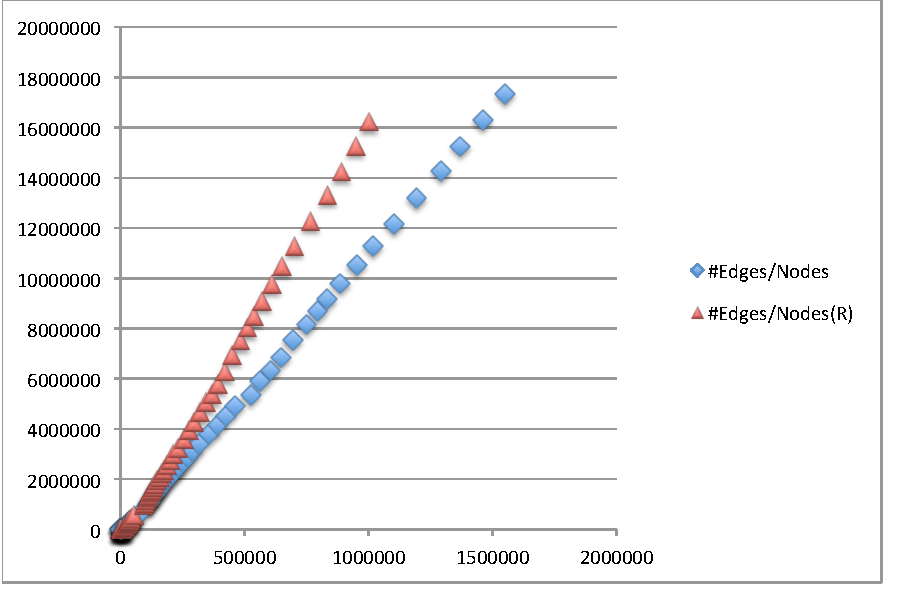
\includegraphics[width=0.3\textwidth]{./graphs/p2-1}
}
\caption{Number of Nodes and Edges over Time \label{fig:growth}}
\end{figure*}

\begin{figure*}
\centering{
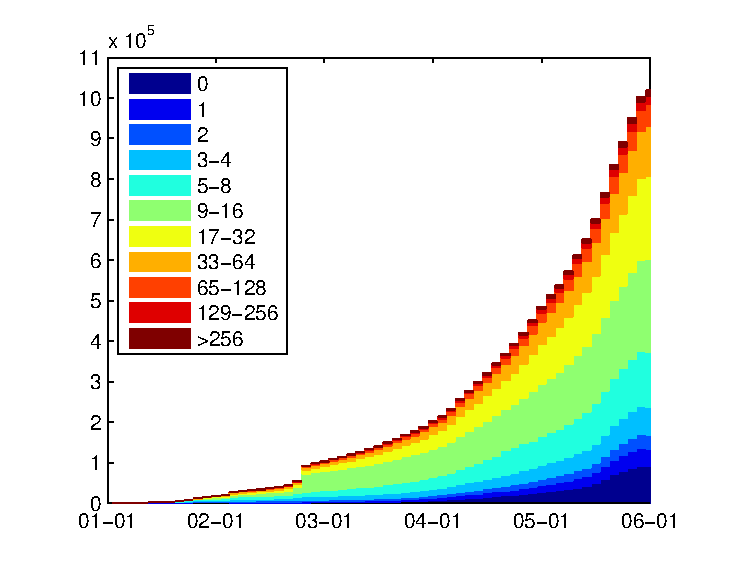
\includegraphics[width=0.33\textwidth]{./graphs/degree}
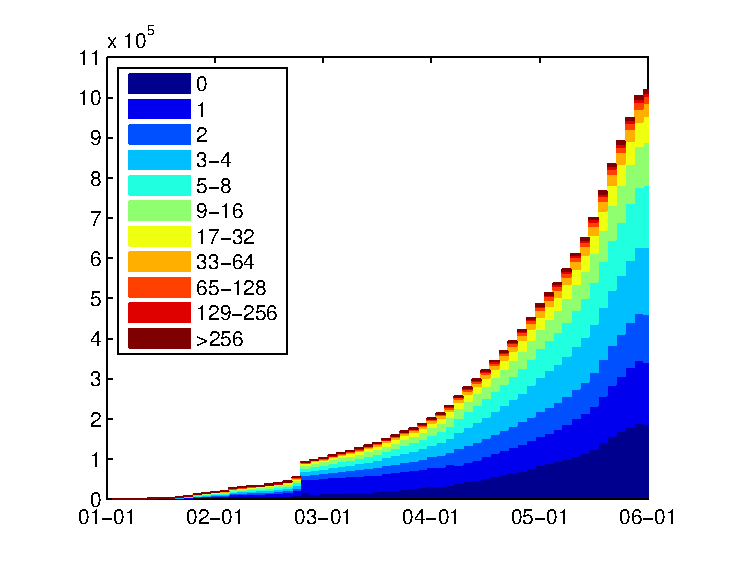
\includegraphics[width=0.33\textwidth]{./graphs/indegree}
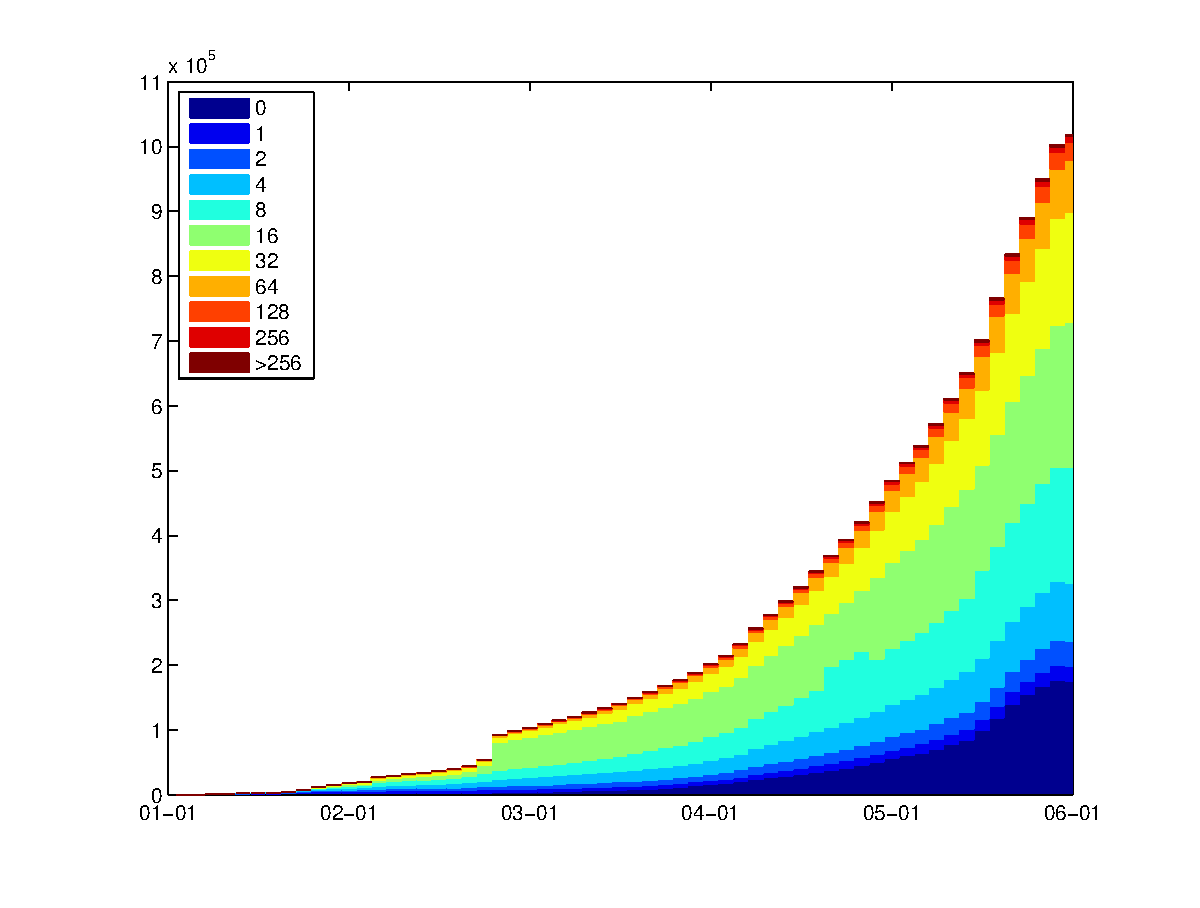
\includegraphics[width=0.33\textwidth]{./graphs/outdegree}
}
\caption{Degree, In-Degree and Out-Degree Distributions over Time \label{fig:degree}}
\end{figure*}

\subsection{Diameter}
As shown in Fig.~\ref{fig:diameter}, the diameter of the graph increases first, and then decreases to a constant range and stabilizes. The initial large diameter might be caused by the disconnectivity of the graph, but the final stabilization shows that the diameter of our Wikipedia network does not increase as its nodes and edges increase, and that Wikipedia is a scale-free network. It is not surprising that after processing redirections, the diameter of the graph shrinks by about 1, the common length of redirection chains.

\begin{figure}[H]
\centering{
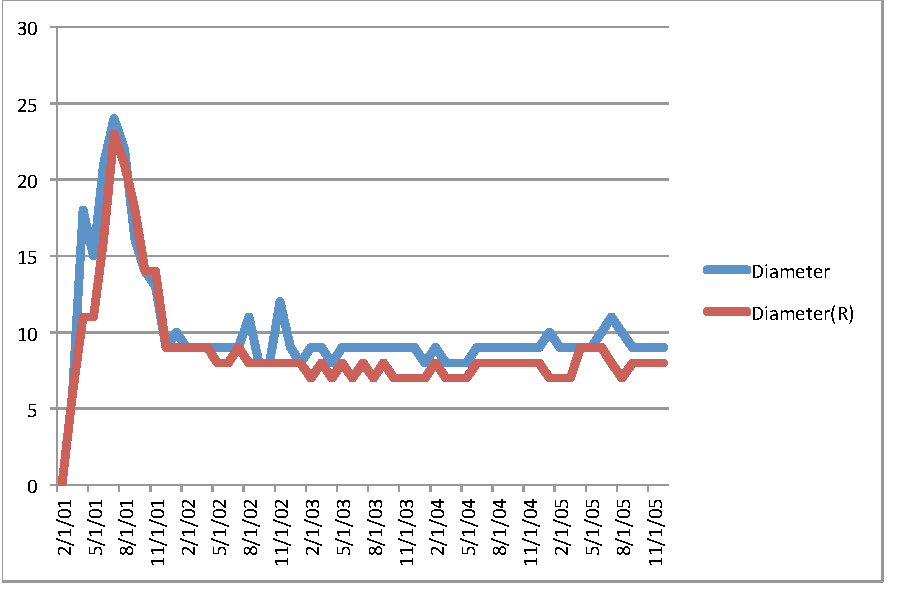
\includegraphics[width=0.8\linewidth]{./graphs/p2-2}
}
\caption{Change of Diameter over Time\label{fig:diameter}}
\end{figure}

\subsection{Connected Component Sizes}
We also looked at Wikipedia's connected component sizes over time. We found that the size of the largest Strongly Connected Component dropped significantly after we removed redirection chains. To investigate this huge difference, we looked at the portion of redirection nodes that were inside the largest SCC. As it turned out, only about 40\% of the nodes removed after processing redirection nodes were from inside the largest SCC, which suggests that redirection pages occur more often in the in-component, out-component, and disjoint component of the network. This lends some insight into the general structure of the Wikipedia network.

\begin{figure}[H]
\centering{
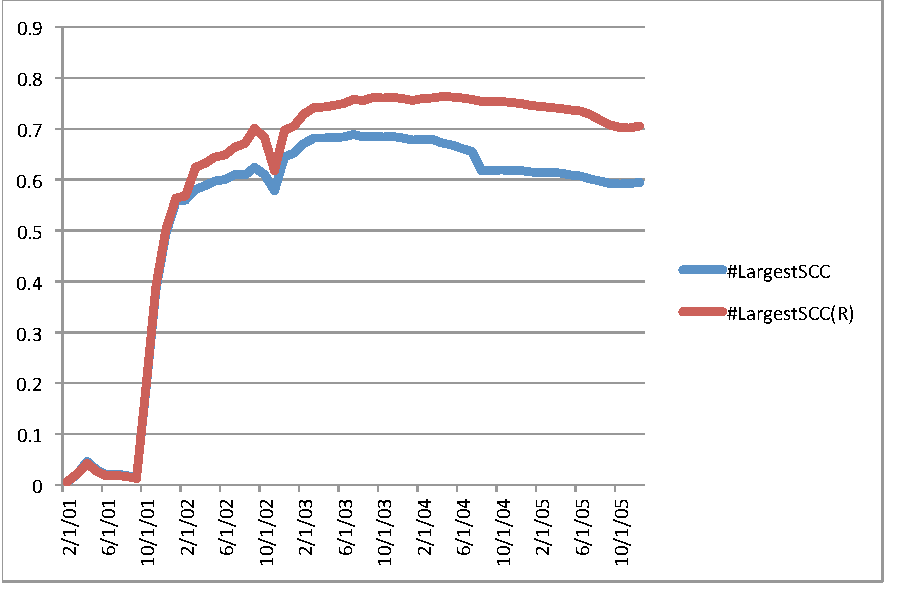
\includegraphics[width=0.5\linewidth]{./graphs/p3-1}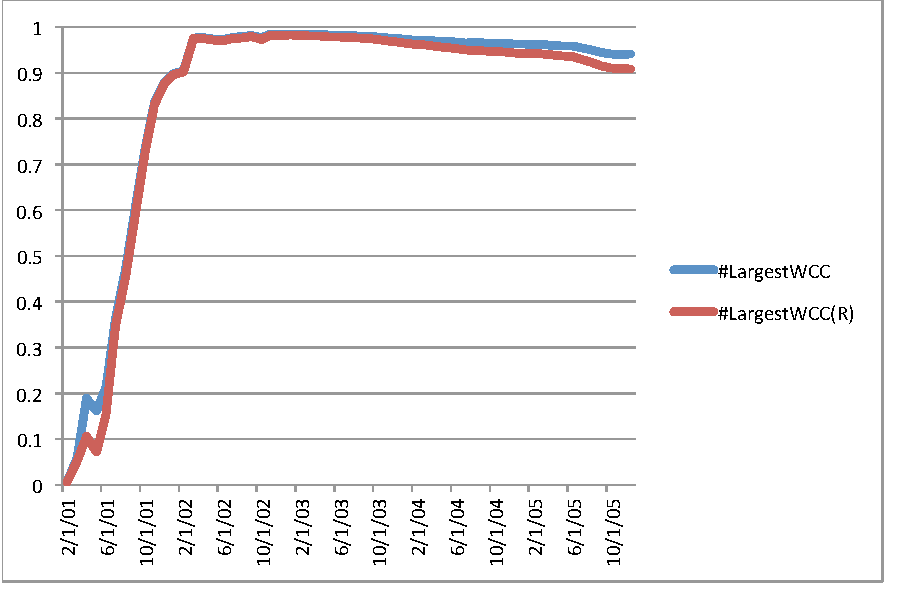
\includegraphics[width=0.5\linewidth]{./graphs/p3-2}
}
\caption{Change of Connected Component Sizes \label{fig:cc}}
\end{figure}

\subsection{Degree Distribution}

REVIEW PENDING

From this point on, we consider only Wikipedia networks with redirection removed. Previous observations has given insight on the effect this process has on the network. It has proved that removing the redirection is a natural process that does not have a major effects on the network.

Fig.~\ref{fig:degree} shows the distribution of degree, in-degree and out-degree of nodes in Wikipedia network over time. Each color represents the number of nodes that fall in a certain range of values. 

From the figures, it appears that the distribution is relatively stable despite the number of nodes grow exponentially. To further investigate Wikipedia's scale-free properties, we drew degree distributions of the Wikipedia network (without aggregation) at certain time points. Fig.~\ref{fig:deg_dist} shows the snapshot on XXXX. It clearly satisfies power law. 

Further, we estimated the $\alpha$ exponent over time. You can find the trend of $\alpha$ in fig.~\ref{fig:alpha_trend}. At the beginning, there were too little nodes and $\alpha$ value is much larger than in common established networks. But $\alpha$ goes down quickly. Within a year since Wikipedia's origin, it is not far away from its current value. $\alpha$ converges to XX. 

\section{Dynamic Analysis}
After we generate snapshots and analyze properties of the whole network, we move on to study the dynamics of the network, namely, the process that determines edge destination.

We study individual edge creation processes in the following way: Note that if we take two snapshots of the network in a short period of time, the vast majority of nodes and edges will not have changed. If the interval is sufficiently short, there will only be a small amount of changes in the network, consisting of creations and deletions of nodes and edges. Since we are not interested in the deletion of nodes and edges, we will only look at the added nodes and edges. In this way, by comparing snapshots, we can single out individual node creations and edge creations. The process of comparing snapshots is shown below:
\begin{figure}[H]
    \centering
        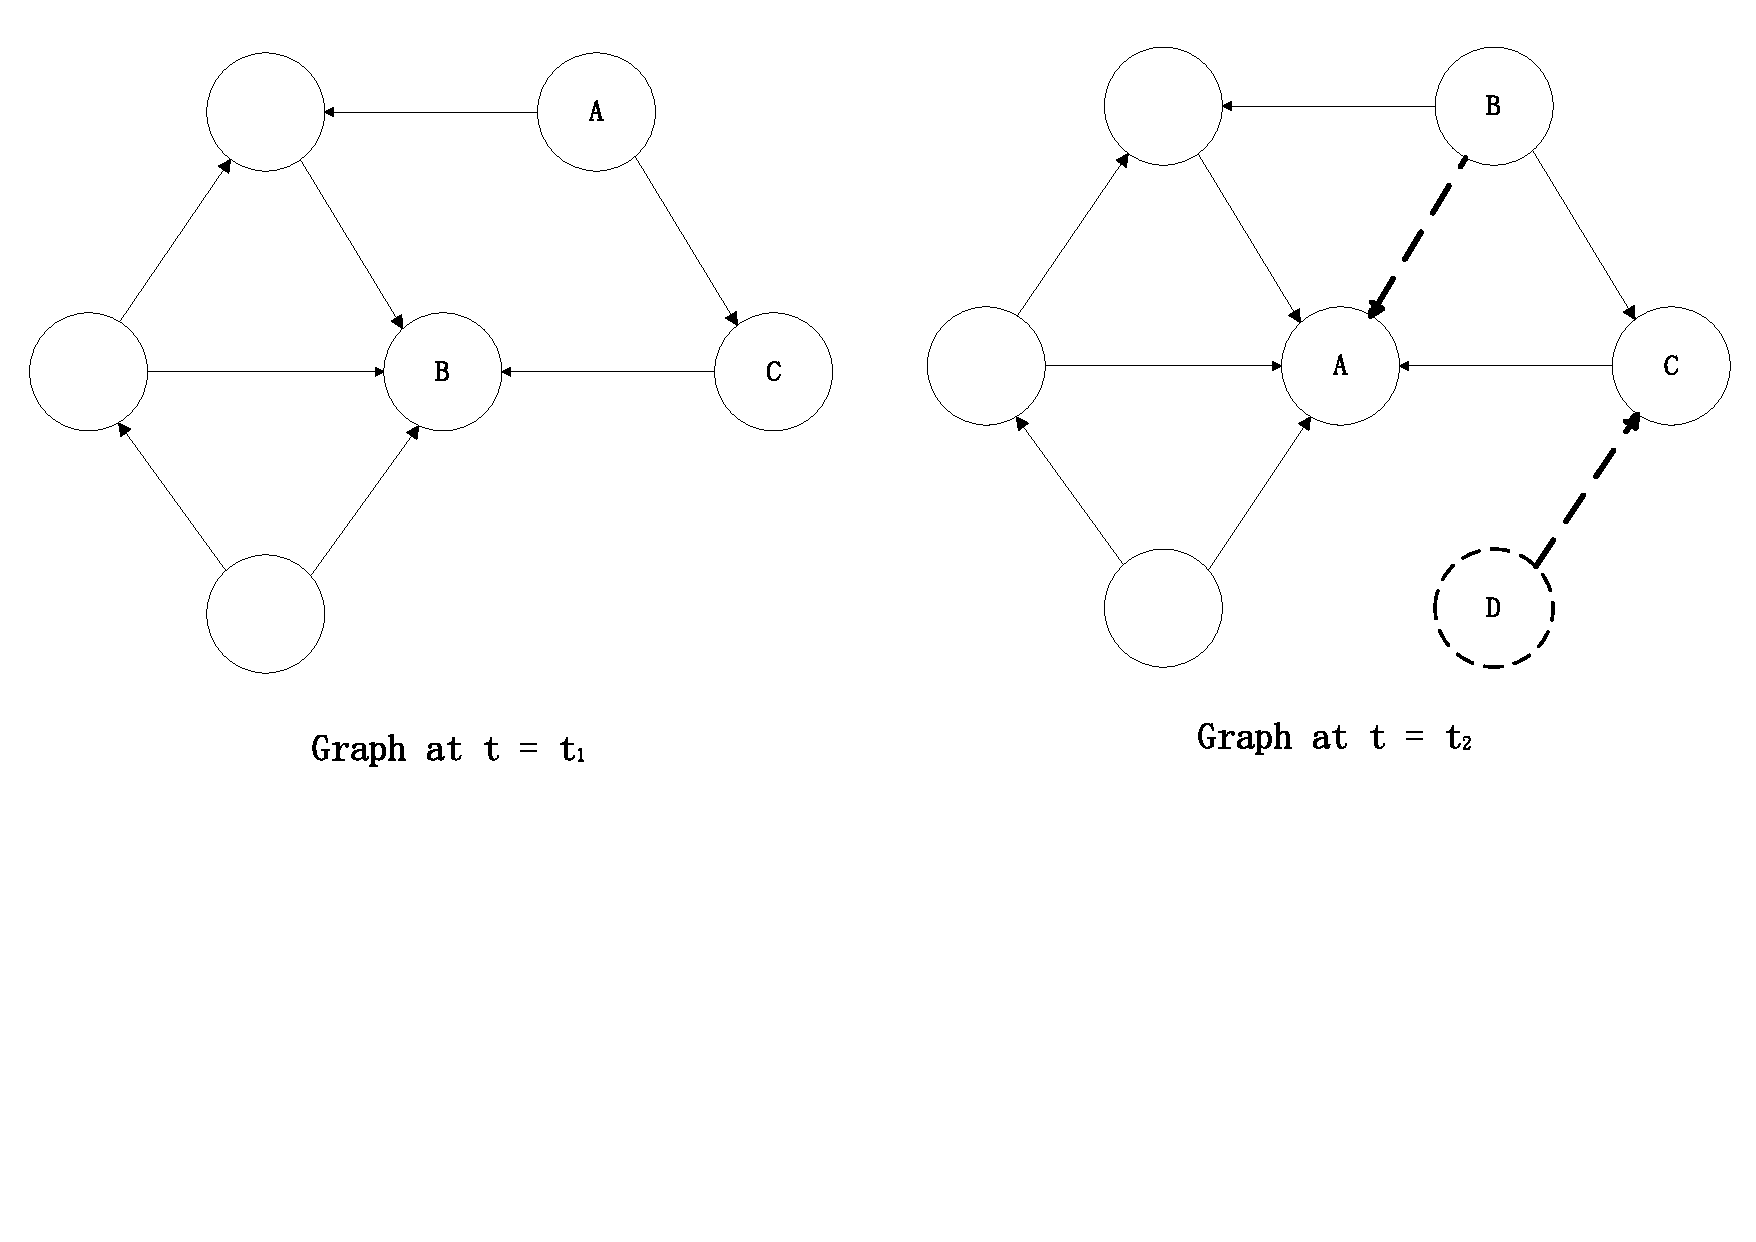
\includegraphics[scale = 0.25, trim = 0cm 8cm 0cm 0cm]{./graphs/dynamic.pdf}
    \caption{Comparing snapshots} \label{fig:compare}
\end{figure}

This process is analogous to taking the derivative of the graph at a certain time. Now, for each observed edge creation, we study it in a dynamic setting. As mentioned earlier, we study the selection of destination, in particular two aspects:
\begin{enumerate}
\item How far away the destination is from the source (Triangle closing model).
\item What are the properties of the destination node (Preferential Attachment model).
\end{enumerate}

\subsection{Triangle Closing}
For the first item, we treat our network as undirected and run depth-limited BFS (Shortest Path would be computationally inefficient) from the source node to determine the number of hops between source and destination. Distance 1 means that the new edge is a reciprocal edge, distance 2 means that the new edge closes a triangle. We look at the proportion of reciprocal edges and triangle-closing edges. Fig.~\ref{fig:portion123} shows the results.
\begin{figure}[H]
    \centering
    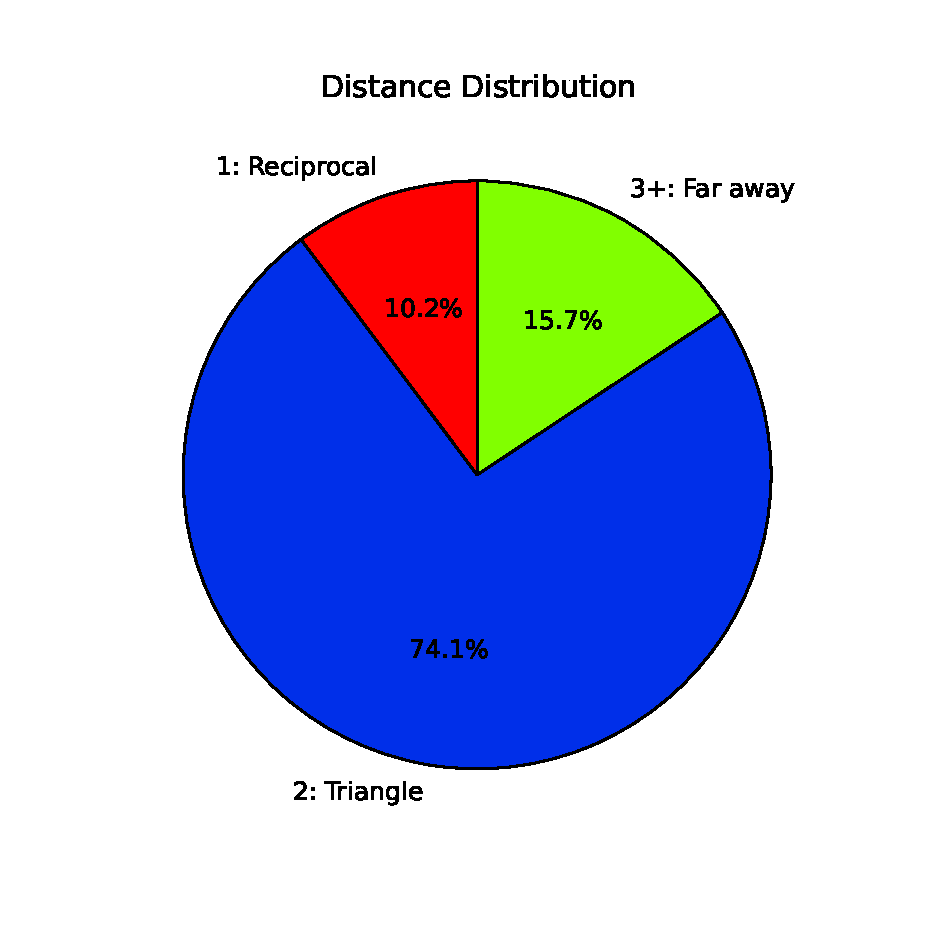
\includegraphics[scale=0.4]{./graphs/distance_pie.eps}
    \caption{Distance between source and destination of new edges} \label{fig:portion123}
\end{figure}
From Fig.~\ref{fig:portion123}, we see that the majority of new edges are between nodes of distance 2, taking up about 70\% of all edges. The result that a large portion of new edges are triangle-closing edges is similar to the findings of \cite{leskovec2008microscopic}. This similarity suggests that both social networks and knowledge networks have this property. Also, the fact that most new edges close triangles makes it more interesting to look into what types of triangles these new edges tend to close.

To study triangle closing for Wikipedia, we generalize the triangle closing theory to directed graphs. Note that the same triangle closing case on an undirected graph can turn into four possible types of cases for a directed graph, as shown below: 
\begin{figure}[H]
    \centering
        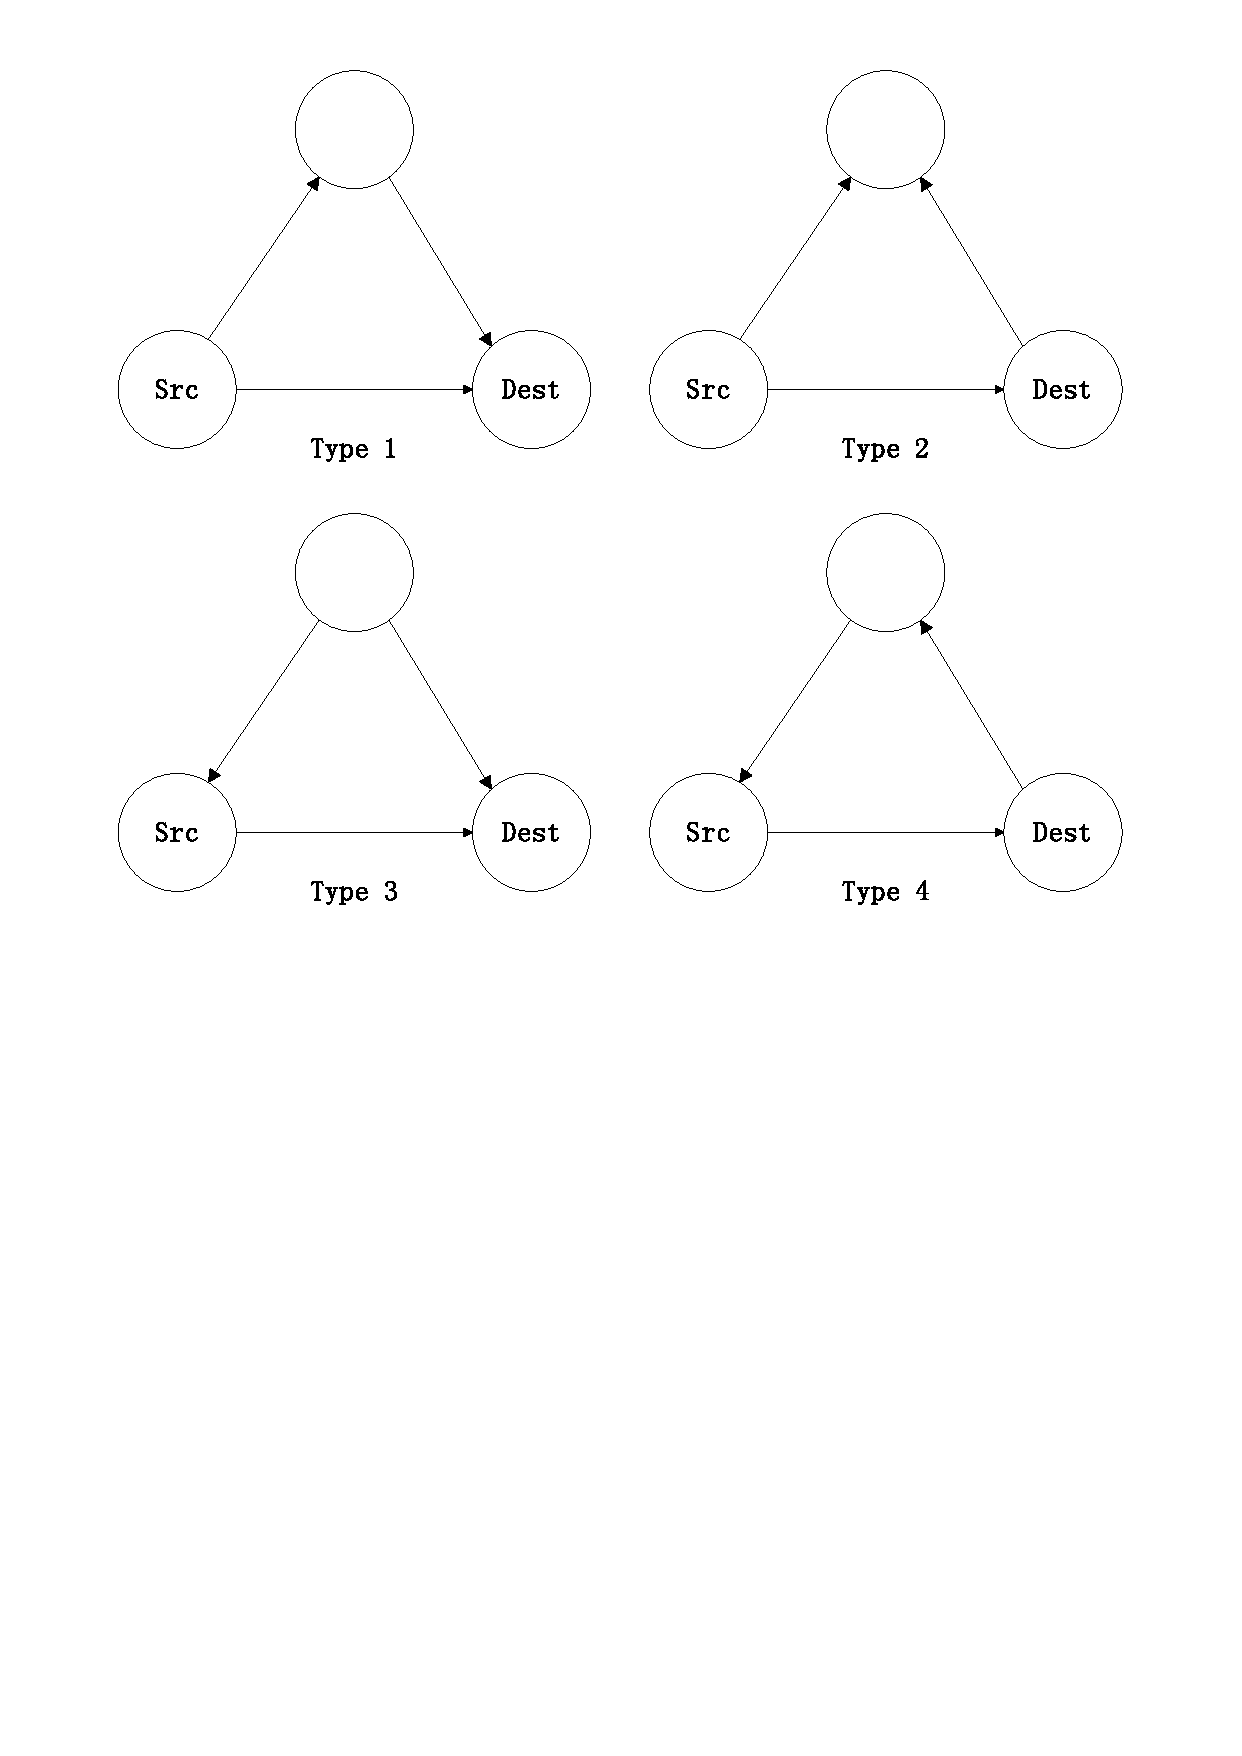
\includegraphics[scale = 0.35, trim = 2cm 14cm 2cm 1cm]{./graphs/triangles.pdf}
    \caption{Types of directed triangles} \label{fig:triangles}
\end{figure}
We look into which kind of triangles the new edges tend to close. Also, note that one single edge may close more than one type of triangle in a directed graph, and there are 15 combinations in all. 
\begin{figure}[H]
    \centering
    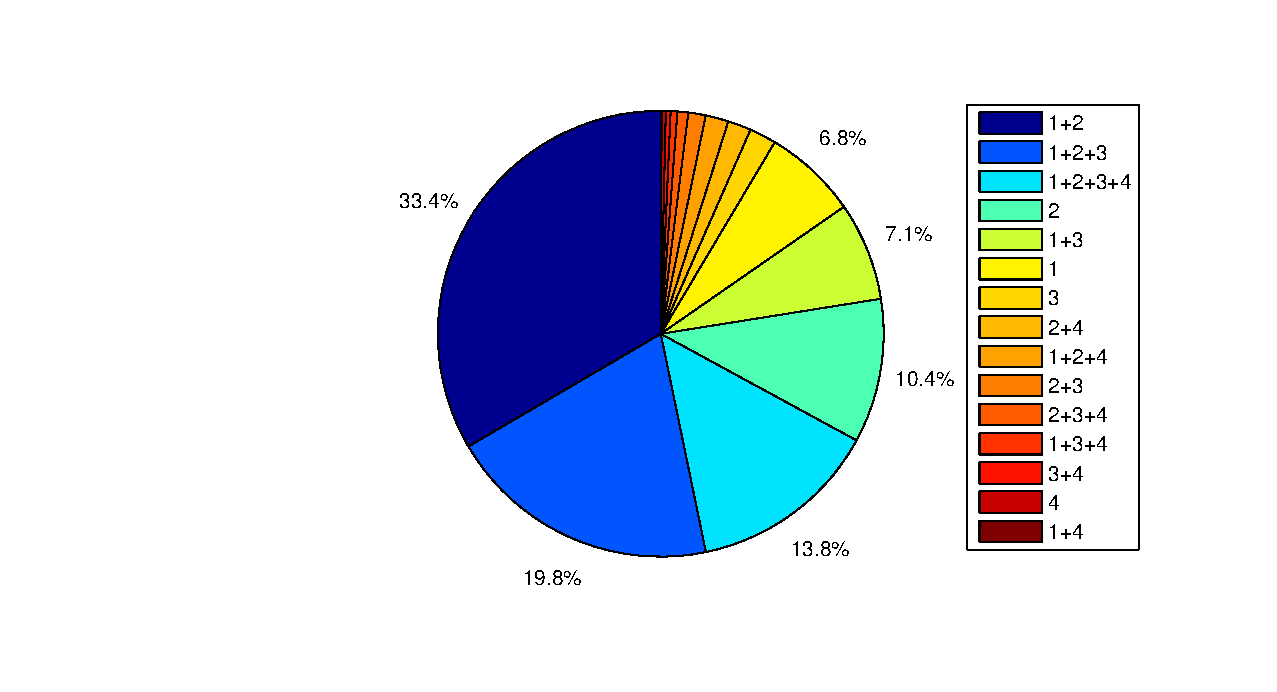
\includegraphics[scale=0.45, trim = 6cm 1cm 0cm 0cm]{./graphs/15_tri.eps}
    \caption{Combination frequency of triangles closed} \label{fig:combo15}
\end{figure}

First, we analyze the four basic types of triangles. Type 1 triangle closing is analogous to creating a `shortcut' in reference. Type 2 and type 3 are new references between `peers', while closing a type 4 triangle creates a cycle of references. 

Aggregating over all cases, type 1 and type 2 triangles are the most popular. However, type 1 triangles often come in combinations with other triangles, while standalone type 2 triangles account for 10\% of all cases, the highest among the four types.

This suggest that shortcut edges are often created, and that shortcuts are more likely when the nodes involved are closely cross-referenced. On the other hand, connections between peers of `reference children' are also common, and the `children' do not need to have back-references from their parents to get connected to each other.

We also see that type 4 triangles are least popular, whether standalone or in combination. Note that closing a type 4 triangle creates a cycle of references. The scarcity of pure cycle references makes sense in a network analysis point of view.

From Fig.~\ref{fig:combo15}, we see that two-thirds of the triangles closed have the combination `1+2', which leads to the following intuition: If node B and node C reference each other, and node A references node B, then node A will likely create a reference to node C as well.

Another popular combination is `1+3', which means that if node A and node B reference each other, and node A points to node C, then node B is likely to generate a new edge also pointing to node C.

The two cases above can be summarized like so: If two Wikipedia nodes reference each other, then they are likely to generate edges pointing to the same node, and are likely to attract edges coming from the same node. We believe that this observation from data makes sense in the real world.

\begin{figure*}
\centering{
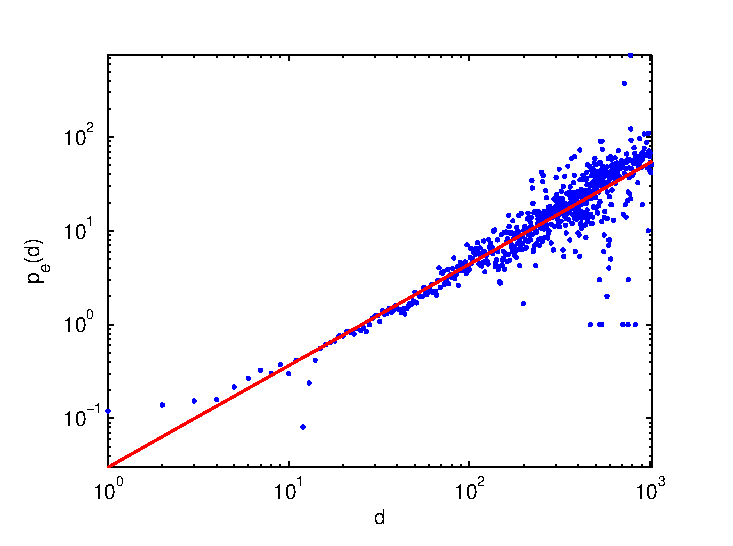
\includegraphics[width=0.32\textwidth]{./graphs/deg_prob}
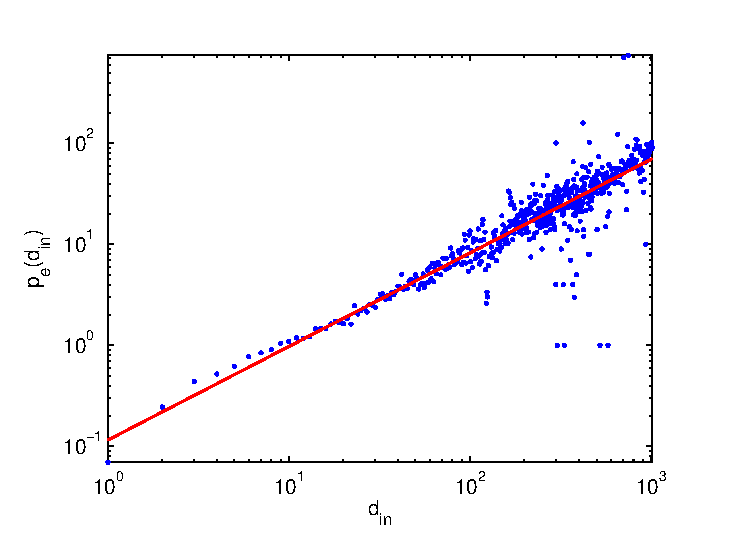
\includegraphics[width=0.32\textwidth]{./graphs/indeg_prob}
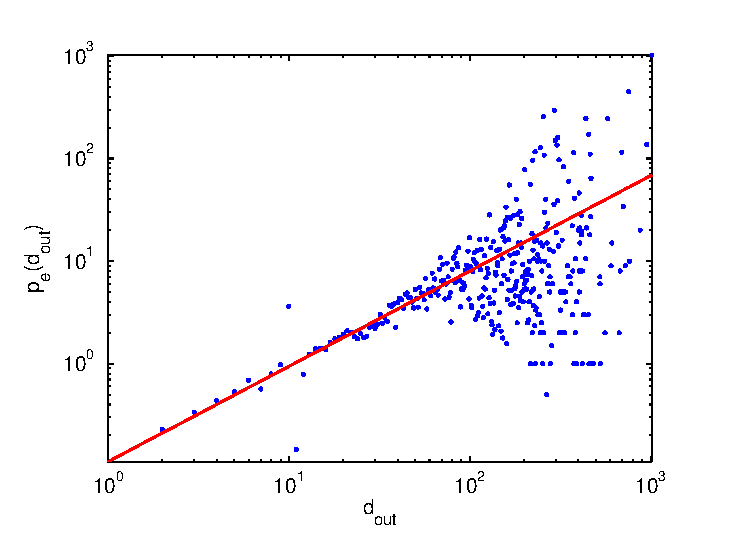
\includegraphics[width=0.32\textwidth]{./graphs/outdeg_prob}
}
\caption{Degree, In-Degree and Out-Degree Distributions over Time \label{fig:degree}}
\end{figure*}

\subsection{Preferential Attachment}
In this section, we study Preferential Attachment(PA) in edge destination selection. The PA model is described as when a new node $j$ joins the network, it creates a constant number of edges, where the edge destination is proportional to the destination's degree.
\begin{equation}
\label{1}
P(j\rightarrow i)=\frac{d_i}{\sum\limits_{k}d_k}
\end{equation}

In \cite{leskovec2008microscopic}, PA was studied as the bias in selection of edge destination based on the degree and age of the node. In the case of degree, the probability of a new edge $e$ choosing a destination of degree $d$ was computed as:
\begin{equation}
\label{2}
p_e(d)=\frac{\sum\limits_{t}[e_t=(u,v)\wedge d_{t-1}(v)=d]}{\sum\limits_{t}|u:d_{t-1}(u)=d|}
\end{equation}

We use the above equation to calculate $p_e(d)$ for edge creation in our Wikipedia graph. If the data was generated by the PA model given in \eqref{1}, we would see that $p_e(d)\propto d$. We fit a parameter $\tau$ to our data so that $p_e(d)\propto d^\tau$. If $\tau \approx 1$, the PA by degree model is further justified on our Wikipedia graph. Our results are shown in the following graph:

From Fig.~ , we see that...

\section{Model Proposal -\\ PA by PageRank}

After evaluating Preferential Attachment by degree on our Wikipedia graph, we go on to propose a PA model of our own. Recall that the original PA model arose from the notation that ``the rich get richer'', with the degree of a node as a measure of importance. It is therefore natural to retain this notion of cumulative advantage, but use a different feature as the measure of importance.

One motivation for trying out another measure of importance arises out of observations from results from previous experiments. In \cite{leskovec2008microscopic}, PA with in-degree was evaluated on some social networks. The findings were that $p_e(d)\propto d$ worked for some networks (for DELICIOUS, $p_e(d)\propto d^{0.9}\approx d$), but for some networks, links did not attach preferentially by degree. In the case of LINKEDIN, we see that $p_e(d)\propto d^{0.6}$ for low degree nodes and $p_e(d)\propto d^{1.2}$ for high degree nodes, suggesting that low degree and high degree nodes get sub-preferential and super-preferential treatment according to their degree, respectively. This leads one to contemplate the possibility that there exists a better measure $m$ for importance than in-degree, so that $p_e(d)\propto m$ fits well to broad cases. 

We propose that the PageRank score of a node may be a good alternative measure of importance. Recall that PageRank conveys the idea that the importance of a node not only depends on the number of links it has, but also depends on the importance of the nodes it is linked to. This appears to be a more robust notion of importance than just the in-degree of a node.

Therefore, we are interested in trying out Preferential Attachment by PageRank. This is done as follows:

First, we compare snapshots with short intervals to single out individual edge creations.~Say we are studying the destination of newly created edge $e$.

Next, we calculate the PageRank scores of nodes in the original graph using the equation below (with other implementation details):
\begin{equation}
\label{3}
r(j)=\sum\limits_{i\rightarrow j}\beta\frac{r(i)}{d_i}+(1-\beta)\frac{1}{n}
\end{equation}

Then, just like how we evaluated PA by node degree, we calculate the probability of a new edge $e$ choosing a destination of PageRank $pr$ as:
\begin{equation}
\label{4}
p_e(pr)=\frac{\sum\limits_{t}[e_t=(u,v)\wedge r_{t-1}(v)=pr]}{\sum\limits_{t}|u:r_{t-1}(u)=pr|}
\end{equation}

(Note that we discretize the PageRank score of nodes so that the results are meaningful.)

Finally, we can plot $p_e(pr)$ against $pr$ to see if there is a relation where $p_e(pr)\propto pr^\tau$, $\tau \approx 1$. Our results are shown in Fig.






As PageRank turned out to be a good measure of importance for Preferential Attachment, we can easily modify the generation model given by \eqref{1}, substituting $\frac{d_i}{\sum\limits_{k}d_k}$ with $\frac{r_i}{\sum\limits_{k}r_k}=r_i$, which gives us
\begin{equation}
\label{5}
P(j\rightarrow i)=\frac{r_i}{\sum\limits_{k}r_k}=r_i
\end{equation}

In this generation model, after the insertion of each node, PageRank needs to be run to modify the new weights. Luckily, we can use values from the previous iteration (warm start) to greatly save computation.

From the preliminary experimental results, we see that one potential problem with the generation model might be that due to the way PageRank is calculated, `rich' nodes might get `too rich' as the network grows. We need to adjust parameters so that we introduce a higher probability of a new node creating random edges, and a lower probability of new edges following probability by PageRank score.

\section{Discussion and Next Steps} 


\bibliographystyle{plain}
\bibliography{ref}
\end{multicols}

\end{document}
